\documentclass[11pt]{beamer}

\usetheme{metropolis}

\usepackage{graphicx}
\usepackage{physics}
\usepackage{adjustbox}
\usepackage{caption}
\usepackage{chemformula}
\usepackage{quoting}
\usepackage[style=chem-angew,backend=bibtex]{biblatex}
\bibliography{references}
%
% Choose how your presentation looks.
%
% For more themes, color themes and font themes, see:
% http://deic.uab.es/~iblanes/beamer_gallery/index_by_theme.html
%
\mode<presentation>
{
  \usetheme{default}      % or try Darmstadt, Madrid, Warsaw, ...
  \usecolortheme{default} % or try albatross, beaver, crane, ...
  \usefonttheme{default}  % or try serif, structurebold, ...
  \setbeamertemplate{navigation symbols}{}
  \setbeamertemplate{caption}[numbered]
  \setbeamerfont{footnote}{size=\tiny}
} 

\usepackage[english]{babel}
\usepackage[utf8]{inputenc}
\graphicspath{{../lectureMW/image/}}

\AtBeginSection[]{
\begin{frame}{Outline}
  \tableofcontents[currentsection]
\end{frame}
}

\title{Review Chapter 3: Naming Compounds}
\institute{Chemistry Department, Cypress College}
\date{Sept 15, 2022}

\begin{document}

\begin{frame}
  \titlepage
\end{frame}

\begin{frame}{Lecture Weekly Agenda}

  \begin{itemize}
  \item Go over homework assignment; present your work
    for 1pt EC
  \item Review Ch 3 - Chemical Compounds
  \item Finish up Ch 3 lect and worksheet
  \item Homework and quiz 3 released Fri, Sept 16 at 3pm
  \item Homework due Fri, Sept 23 at 11:59pm
  \item Quiz 3 due Tues, Sept 20 at 11:59pm
  \item \textbf{Heads up:} Exam 1 coming up Sept 27 in lecture
    and 1.5 hours exam
  \end{itemize}
\end{frame}

\section{Review: Naming Compounds}

\begin{frame}{Naming Binary Ionic Compounds}
  The metal cation is named first, followed by the nonmetal anion.
  The word ion is dropped from both parts.

  \centering
  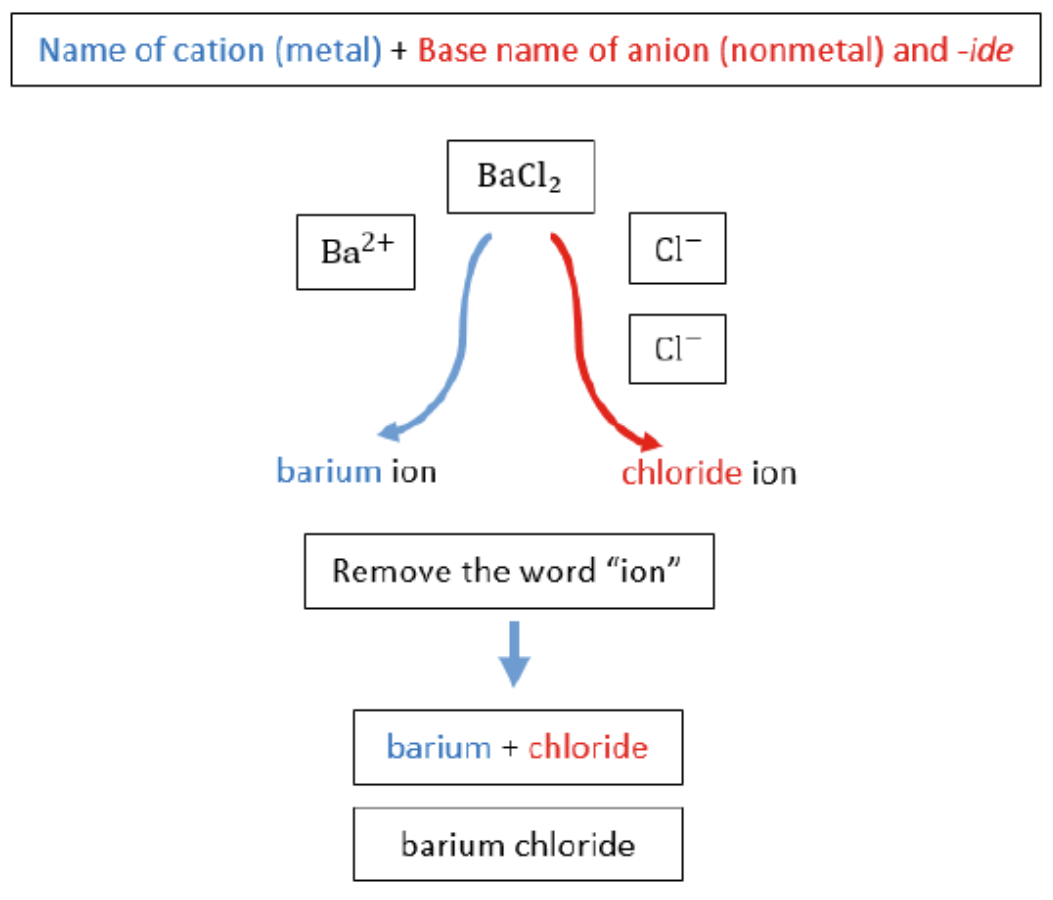
\includegraphics[width=0.7\linewidth]{barium_examp.png}
\end{frame}

\begin{frame}{Naming Molecular Compounds}
  \begin{center}
    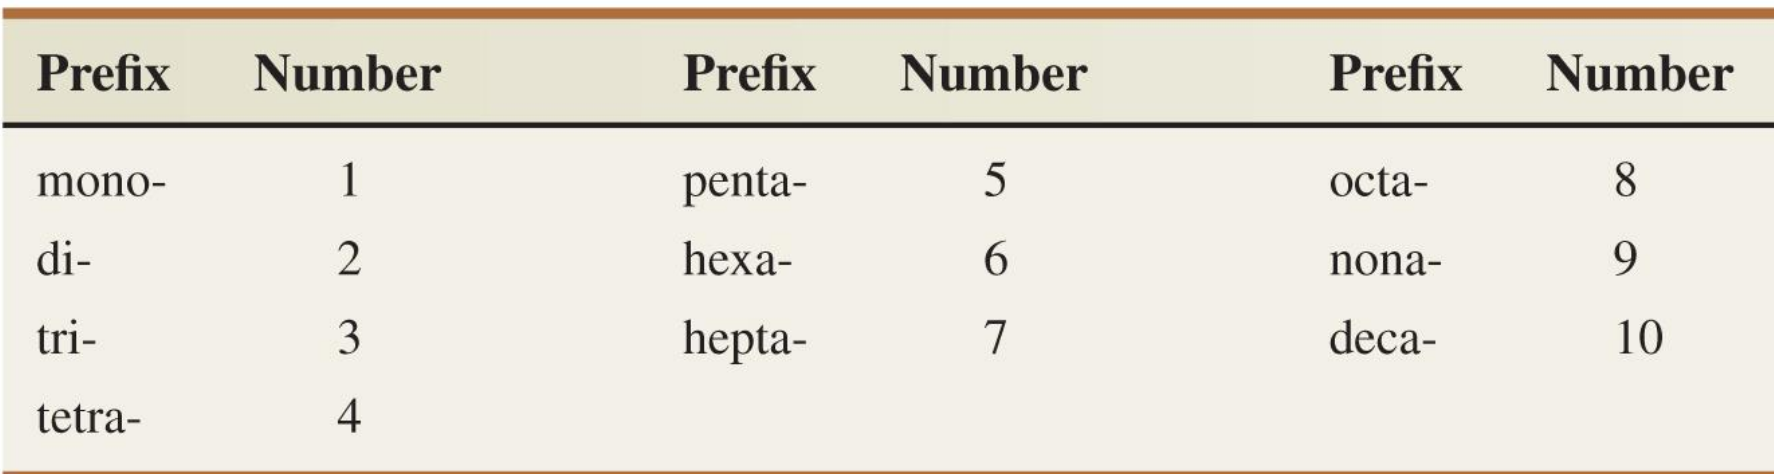
\includegraphics[width=\linewidth]{prefix_name}
  \end{center}
  
  \begin{enumerate}
  \item Use numerical prefix for the element (usually ignore the first
    when using ``mono'')
  \item Add ``-ide'' to the second element
  \end{enumerate}
\end{frame}

\begin{frame}{Naming Acids}
  \begin{center}
    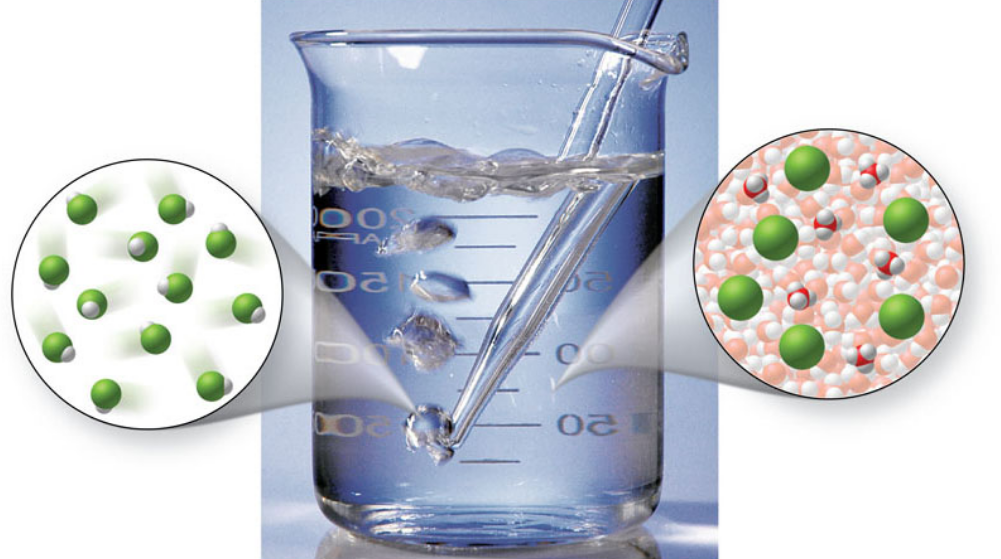
\includegraphics[width=0.5\linewidth]{acid_base}
  \end{center}

  \begin{enumerate}
  \item If anion ends in ``-ide,'' add ``hydro'' before the
    root of the anion name followed by ``-ic acid''
  \item If anion ends in ``-ate,'' use the root of the anion
    name followed by ``-ic acid''
  \item If anion ends in ``-ite,'' use the root of the anion
    name followed by ``-ous acid''
  \end{enumerate}
\end{frame}

\begin{frame}{What is an Acid?}
  \vspace{0.2in}
  \textbf{Arrhenius Acid} - dissociation of acid in water to yield
  the ions e.g. HCl(aq) $\rightarrow$ H$^+$(aq) + Cl$^-$(aq)
  
  \textbf{Br{\o}nsted Acid} - any species that can donate a proton
  H$^+$

  \begin{center}
    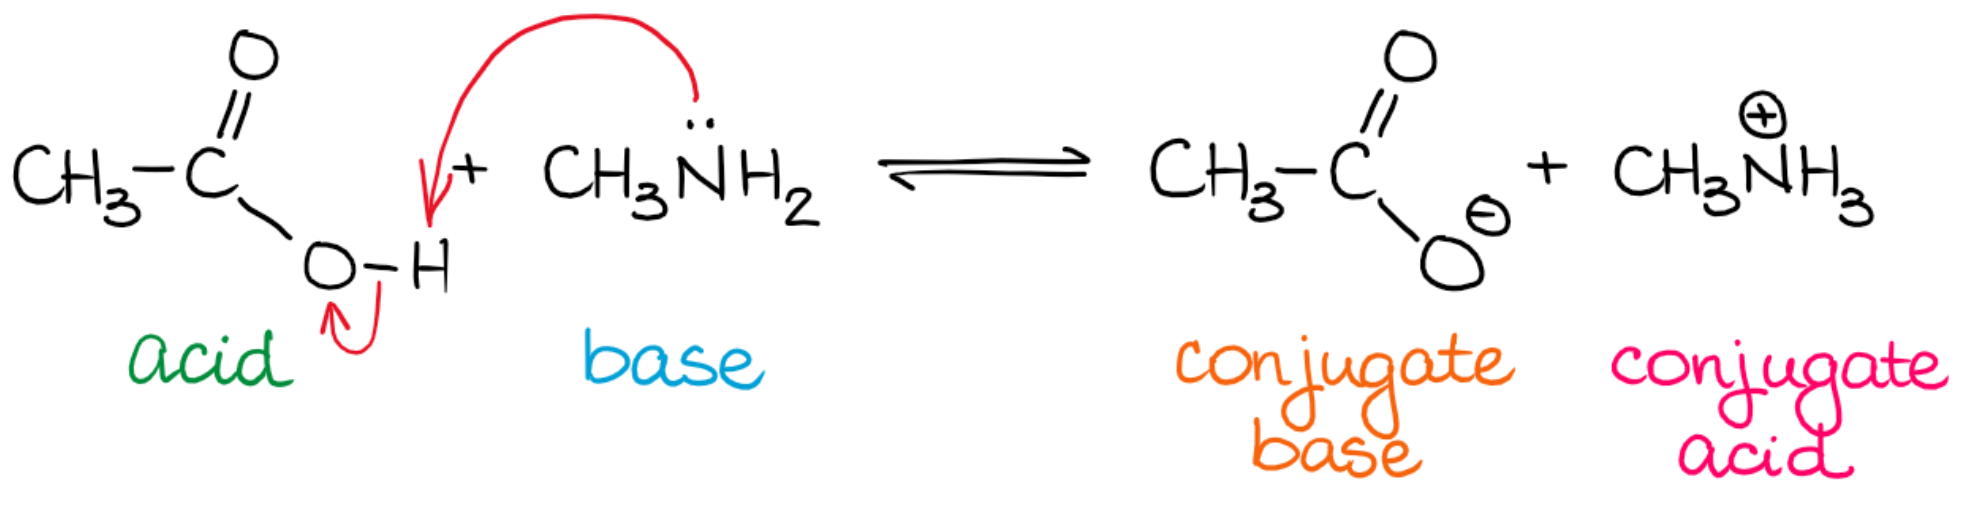
\includegraphics[scale=0.1]{bronsted_acid}
  \end{center}
  \vspace{-0.2in}
  \textbf{Lewis Acid} - donation of a pair of electrons
  \begin{center}
    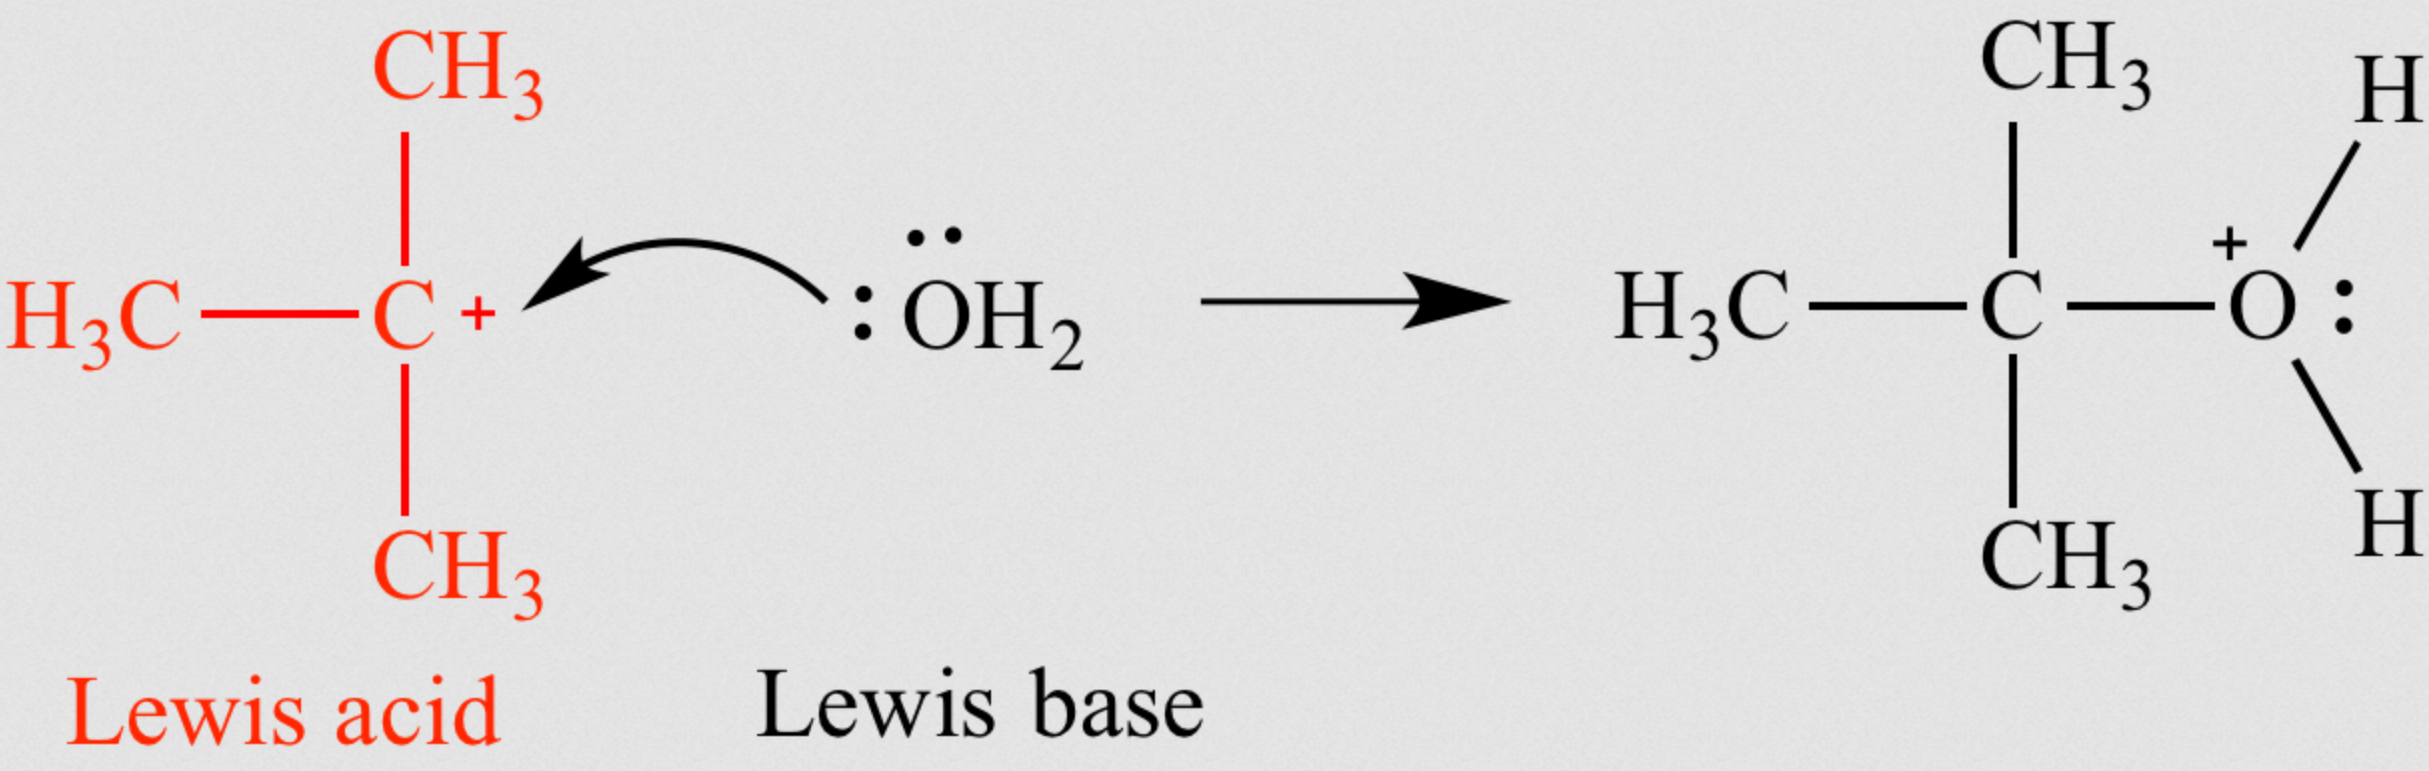
\includegraphics[scale=0.07]{lewis_acid}
  \end{center}
\end{frame}

\end{document}
